\section{Lubrication Physics, Models and Degradation Mechanisms}
\label{sec:lubrication_physics}
Multiple theoretical models of lubrication exist which seek to estimate the lubrication film thickness in running ball bearings and the sufficiency thereof under specific operating conditions and with different lubricants. However, a complete understanding and model of the physico-chemical properties of lubricants and the lubricant film formation in ball bearings has yet to be formulated \cite{cen_ehl_2021} \cite{dai_situ_2024} \cite{li_lubrication_2026}.

The following subsections present the theoretical models most commonly used in LCM research and the degradation mechanisms that affect lubrication conditions. The theoretical models serve two distinct roles: they provide the physics-based reference against which sensor measurements are calibrated, and they establish which physical quantities -- film thickness, friction, heat generation, and elastic wave emission -- can in principle be observed by each class of sensing method. This connection between lubricant physics and observable signal is the foundation for understanding which signal processing operations are meaningful for each modality. The degradation mechanisms are important for understanding the physical origins of signals and the specific monitoring targets that signal processing methods should be optimised for.

\subsection{Lubrication Regimes}
\label{subsec:lubrication_regimes}
Lubrication films formed in ball bearings under operation are generally classified into three regimes depending on the physical contact between balls and raceways and how the bearing load is distributed:
\begin{itemize}
    \item \textbf{Boundary lubrication}: the entire load is carried by surface-to-surface contact (ball to raceway). This regime produces the highest friction, arising solely from sliding of asperities against each other. Wear rate is high, and heat generation and elastic stress-wave emission are correspondingly intense.
    \item \textbf{Mixed lubrication}: load is shared between a thin lubricant film and surface asperity contacts. Friction and wear are reduced compared to the boundary regime but asperity contacts continue to generate transient stress waves detectable by acoustic and vibration sensors.
    \item \textbf{Elastohydrodynamic lubrication (EHL)}: all load is carried by a lubricant film between the balls and raceway. The high pressure building up in the contact zone causes elastic deformation of the solid materials, sustaining the film. Friction is at its minimum for full-film EHL and rises again at excessive viscosities due to viscous shear losses. Wear is minimal and elastic wave emission is negligible, making this the ideal operating regime for bearing longevity.
\end{itemize}
The progression through these regimes as lubrication conditions deteriorate determines both the nature and the intensity of the signals accessible to passive sensing methods.

\subsection{The Stribeck Curve and Its Significance for Signal Processing}
\label{subsec:stribeck}
\todo{Include figure with the Stribeck curve} The Stribeck curve describes the relationship between the friction coefficient and the Hersey number $\eta n / p$, where $\eta$ is the dynamic viscosity, $n$ is the rotational speed, and $p$ is the contact pressure. As the Hersey number decreases -- due to lower speed, lower viscosity, or higher load -- the bearing transitions from the EHL regime, through mixed lubrication, into boundary lubrication, and the friction coefficient rises sharply. The curve is illustrated in Figure~\ref{fig:stribeck}

\begin{figure}[htbp]
    \centering
    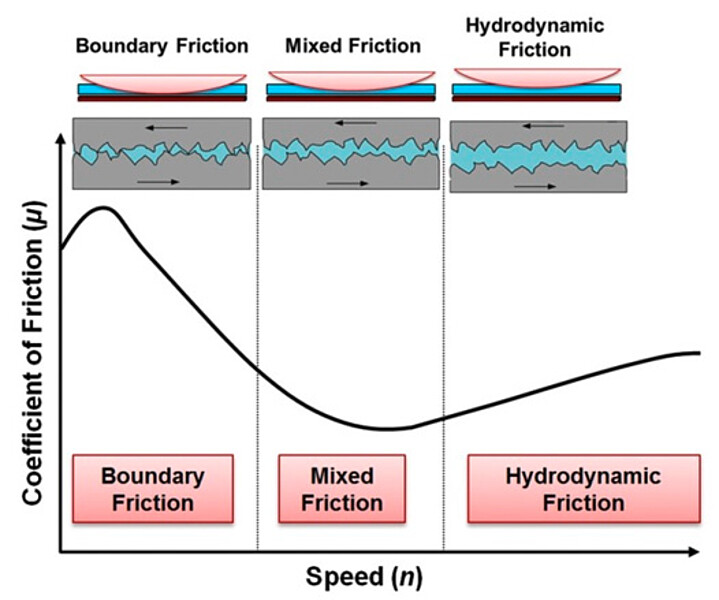
\includegraphics[width=0.5\textwidth]{figures/stribeck_curve.jpg}
    \caption{Stribeck curve illustrating the relationship between friction coefficient and Hersey number, with lubrication regimes indicated.}
    \label{fig:stribeck}
\end{figure}

The Stribeck curve is directly relevant to signal processing because the friction coefficient governs the amplitude of signals detectable by passive methods: higher friction produces stronger elastic wave emission (detectable by acoustic emission and ultrasound sensors), higher heat generation (detectable by temperature and infrared sensors), and increased mechanical vibration (detectable by accelerometers and microphones). A bearing operating in the EHL regime near the Stribeck minimum will produce weaker passive signals than one in boundary lubrication. This has two important signal processing consequences: first, monitoring under optimal lubrication (and in a neighbourhood of the optimum) is inherently a low-SNR problem; second, any feature that is strongly correlated to friction can in principle serve as a lubrication condition indicator. Hou and Zhang \cite{hou_-situ_2025} demonstrate this explicitly by mapping acoustic emission amplitude and energy onto lubrication regime clusters, with the joint distribution in a two-dimensional (amplitude, energy) space discriminating boundary, mixed, and EHL conditions.

\subsection{Hamrock--Dowson Model}
\label{subsec:hamrock_dowson}
The Hamrock--Dowson model is the most widely used empirical model for calculating the central film thickness, $h_m$, in ball bearings. It is given by
\begin{equation}
    \frac{h_m}{R_{x}^{'}} = 3.63\,U^{0.68}\,G^{0.49}\,W^{-0.073}\,(1-e^{-0.68k}),
\end{equation}
where
\begin{itemize}
    \item $R^{'}_{x}$ and $R^{'}_{y}$ are the effective radii in the direction parallel and transverse to the lubricant entrainment, respectively,
    \item $U=\eta_0 u_e/(E^{'}R^{'}_{x})$ is a dimensionless speed parameter, with $u_e$ the lubricant entrainment speed and $E^{'}$ the effective elastic modulus,
    \item $W=w_z/(E^{'}{R^{'}_{x}}^{2})$ is a dimensionless load parameter, with $w_z$ the applied normal load,
    \item $G=\alpha^*E^{'}$ is a dimensionless material parameter, with $\alpha^*$ the pressure-viscosity coefficient, and
    \item $k=1.03(R_{y}^{'}/R_{x}^{'})^{2/\pi}$ is the elliptic parameter.
\end{itemize}
Further derivation and physical motivation of these parameters can be found in \cite{cen_ehl_2021,hansen_new_2021,maruyama_lubrication_2019,noauthor_elasto-hydrodynamic_1977}. In the LCM context, the Hamrock--Dowson model is most often used not to predict film thickness directly, but to generate reference values of $h_m$ against which sensor-derived estimates can be calibrated \cite{jakobsen_detecting_2023,hou_-situ_2025,jablonka_quantitative_2018}.

\subsection{$\Lambda$-Ratio}
\label{subsec:lambda}
The $\Lambda$ ratio is the ratio between the lubrication film thickness and the composite surface roughness of the bearing components, and is widely used to assess the lubrication regime. It is defined as
\begin{equation}
\Lambda = \frac{h_{m}}{\sqrt{R_{q1}^2 + R_{q2}^2}},
\end{equation}
where $h_{m}$ is the minimum film thickness and $R_{q1}$, $R_{q2}$ are the root-mean-square roughness values of the two contacting surfaces. Lubrication regimes are conventionally assigned as: $\Lambda < 1$ (boundary), $1 \leq \Lambda \leq 3$ (mixed), $\Lambda > 3$ (EHL). The $\Lambda$ ratio is the primary physical target variable in some LCM studies that use sensor signals to estimate the lubrication regime \cite{jakobsen_detecting_2023,hou_-situ_2025,cornel_condition_2021}.

Hansen et al.\ \cite{hansen_new_2021} note that the conventional $\Lambda$ ratio has shortcomings in the EHL regime arising from elastic asperity deformation, and propose an improved $\Lambda^*$ ratio:
\begin{equation}
\Lambda^* = \frac{h^*}{z_0} = \frac{h_m+\delta_a}{z_0},
\end{equation}
where $\delta_a$ is the elastic asperity deformation in EHL and $z_0$ is the relaxed-state height of the surface profile.

\subsection{$\kappa$-Ratio}
\label{subsec:kappa}
The $\kappa$ ratio is a model-based indicator of lubricant viscosity adequacy for a specific bearing under specific operating conditions. It is defined as
\begin{equation}
\kappa = \frac{\nu}{\nu_{1}},
\end{equation}
where $\nu$ is the kinematic viscosity of the applied lubricant under the operating conditions and $\nu_{1}$ is the reference kinematic viscosity calculated from the ISO 281 standard for the bearing diameter and rotational speed \cite{jakobsen_detecting_2023}. Interpretation guidelines are:
\begin{itemize}
    \item $\kappa \leq 0.1$: insufficient lubrication; load carried almost entirely by asperity contact.
    \item $0.1 < \kappa \leq 1$: insufficient lubrication; metallic surface-to-surface contact present.
    \item $1 < \kappa \leq 4$: adequate lubrication.
    \item $4 < \kappa$: excessive viscosity; higher viscous friction losses.
\end{itemize}
Given the fact that $\kappa$ can be tied to lubrication conditions it can also be tied to the Stribeck curve and lubrication regimes. The $\kappa$ ratio is related to the $\Lambda$ ratio approximately as $\kappa \approx \Lambda^{1.3}$. Jakobsen et al.\ \cite{jakobsen_detecting_2023,jakobsen_vibration_2021} use $\kappa$ as the regression target for data-driven models trained on vibration and ultrasound features, linking directly to the ISO standard and enabling quantitative LCM without invasive lubricant sampling. It should be noted that $\kappa$ is time-invariant for a given bearing and operating condition; it therefore captures viscosity inadequacy if the conditions remain constant but does not account for lubricant degradation or contamination that develops over time.



\subsection{Lubricant Degradation Mechanisms}
\label{subsec:degradation}For oil-lubricated bearings, degradation proceeds primarily through: thermal and oxidative aging (which increases viscosity temporarily, then reduces it as polymer chains break down), contamination by wear particles or external debris, and oil starvation from insufficient supply or replenishment. For grease-lubricated bearings the degradation picture is more complex. Grease consists of a base oil held in a thickener matrix; degradation involves base-oil bleed-out (reducing available lubricant), mechanical working of the thickener (reducing consistency and channelling behaviour), thermal degradation (affecting both base oil and thickener), and contamination \cite{lugt_grease_2012,sahu_grease_2022,zhang_grease_2021}. Cen et al.\ \cite{cen_effect_2025} specifically study the effect of thermal aging on grease film thickness in ball bearings and show measurable film thickness reduction with aging time. These differing degradation mechanisms mean that signal processing pipelines tuned to detect oil starvation may not transfer directly to grease monitoring applications and vice versa, a gap explicitly identified in Section~\ref{sec:gaps}.

